\documentclass[10pt,a4paper]{article}
\usepackage[utf8]{inputenc}
\usepackage{amsmath}
\usepackage{amsfonts}
\usepackage{amssymb}
\usepackage{graphicx}
\usepackage{verbatim}
\usepackage{float}
\usepackage{tikz}
\usepackage{subfig}
\usepackage{tcolorbox}
\usepackage{parskip}
\usepackage[left=2cm,right=2cm,top=2cm,bottom=2cm]{geometry}
\author{Songtuan Lin u6162630}
\title{Computer Network}
\begin{document}
\maketitle

\section{Basic Terminology}
Network, particularly in terms of Computer Science, is consist of several devices that are able to \textit{communicate} with each other. The term \textit{communicate} here means the device within Network can send or receive message from other devices. In order to perform this communication, each device within Network must be able to be located, or simply speaking, each device must have a \textit{address}. There are several methods to assign \textit{addresses} to devices, each of them corresponding to a specific technology that is used to construct Network. One popular technology is \textit{Internet}, which assign a \textit{IP} to each device within Network as their address. In here, \textit{Internet} is the technology that used to construct Network and \textit{IP} is the method that Internet used to address(locate) devices within it. 

Furthermore, in order to let devices within Network communicate with each other, one essential requirement is that there must be a thing that can carry the message and deliver it between devices. Such thing, which can be called as \textit{media}, consist the \textit{Physical Layer} of Computer Network

\section{Physical Layer}
As described in last section, \textit{Physical Layer} is consist of the media that can carry and deliver messages. Particularly, as Figure \ref{physical_layer} illustrated, the media is the line that connect Device A and B. 
\begin{figure}[ht]
	\center
	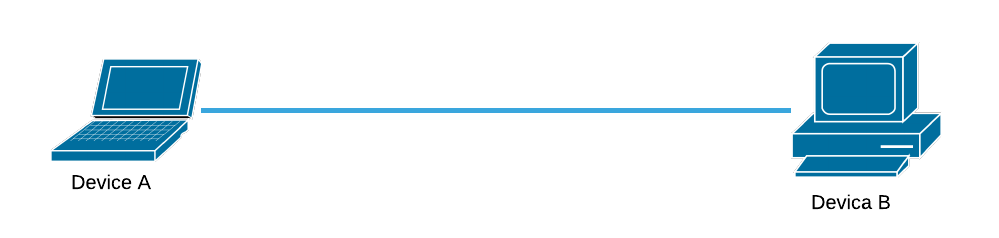
\includegraphics[scale=0.85]{Physical}
	\caption{Media between Different Devices}
	\label{physical_layer}
\end{figure}
Furthermore, based on the characteristics of the media, it can be categorized into following three classes::
\begin{enumerate}
	\item \textbf{Simplex}: This type of media can only transport message with a \textit{fixed direction}, \textsl{e.g.} from Device A to Device B.
	\item \textbf{Half-Duplex}: This type of media can transport message with both directions. However, it can only choose one direction during each transportation, \textsl{e.g.} from A to B or B to A.
	\item \textbf{Duplex}: This type of media can transport message with both direction during a transportation, \textsl{e.g.} transport message from A to B and B to A in the same time.
\end{enumerate}
Indeed, the Figure \ref{physical_layer} give us an inspiration about how to construct a simple network, which is connecting each devices within network with a media. For example. assume we want to construct a Network contain four devices, the easiest way to do this is shown in Figure \ref{topology_basic}, in which, each device is connected with the rest.
\begin{figure}[H]
	\center
	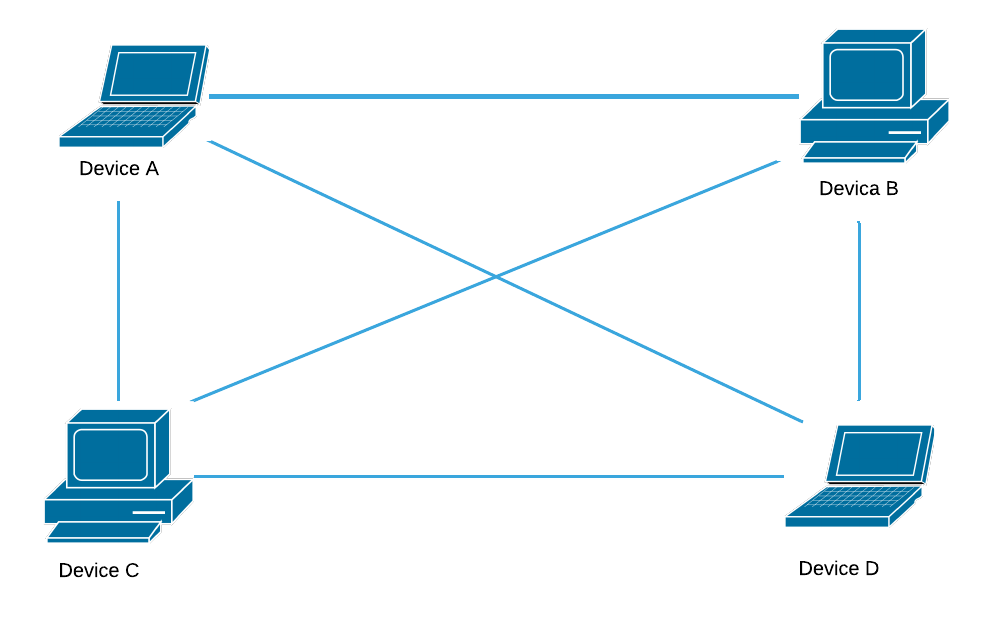
\includegraphics[scale=0.5]{Topology}
	\caption{Basic Topology}
	\label{topology_basic}
\end{figure}
However, the problem of this topology is that the number of medias will grow exponentially with the increasing number of devices. Therefore, an improvement topology along with an algorithm(protocol) to control how the messages are delivered is required, which relate to our next topic: \textit{Data-Link Layer}

\section{Data-Link Layer}
The solution of the problem remaining in last section is straightforward: By adding one or more \textit{Switch} which depend on the number of devices within network. The Switches work as bridges that connect different devices in Network, as illustrated in Figure \ref{topo}:
\begin{figure}[H]
\center
\subfloat[]{\begin{tikzpicture}
	\node[label=below:Device] (laptop_1) at (6, 3){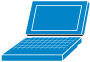
\includegraphics[scale = 0.3]{laptop}};
	\node[label=below:Switch] (switch) at (3, 3){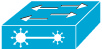
\includegraphics[scale = 0.3]{switch}};
	\node[label=below:Device] (laptop_2) at (0, 3){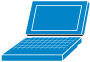
\includegraphics[scale = 0.3]{laptop}};
	\node[label=right:Device] (laptop_3) at (3, 1){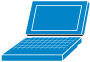
\includegraphics[scale = 0.3]{laptop}};
	\node[label=right:Device] (laptop_4) at (3, 5){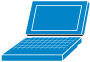
\includegraphics[scale = 0.3]{laptop}};
	
	\draw[blue, thick] (laptop_1) -- (switch);
	\draw[blue, thick] (laptop_2) -- (switch);
	\draw[blue, thick] (switch) -- (laptop_3);
	\draw[blue, thick] (switch) -- (laptop_4);
\end{tikzpicture} \label{topo_1}} \\

\subfloat[]
{
	\begin{tikzpicture}
		\node[label=below:Device A] (laptop_1) at (1, 4){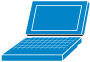
\includegraphics[scale=0.3]{laptop}};
		\node[label=below:Device B] (laptop_2) at (1, 2){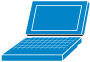
\includegraphics[scale=0.3]{laptop}};
		\node[label=below:Switch A] (switch_1) at (3, 3){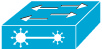
\includegraphics[scale=0.3]{switch}};
		\node[label=below:Switch B] (switch_2) at (5, 3){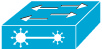
\includegraphics[scale=0.3]{switch}};
		\node[label=below:Device C] (laptop_3) at (7, 4){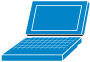
\includegraphics[scale=0.3]{laptop}};
		\node[label=below:Device D] (laptop_4) at (7, 2){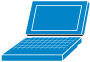
\includegraphics[scale=0.3]{laptop}};
		
		\draw[blue, thick] (laptop_1) -- (switch_1);
		\draw[blue, thick] (laptop_2) -- (switch_1);
		\draw[blue, thick] (switch_1) -- (switch_2);
		\draw[blue, thick] (switch_2) -- (laptop_3);
		\draw[blue, thick] (switch_2) -- (laptop_4);
	\end{tikzpicture}
	\label{topo_2}
}
\caption{Two Example of Network Topology}
\label{topo}
\end{figure}
Even though the switches reduce the number of connection, the new problem is how the the different devices communicate with each other under the condition that they are not direct connected. This problem may be better illustrated by an example: Assume Device A in Figure \ref{topo_2} is willing to send a message to Device D. The first thing Device A need to do is locating Device D, or we can say, Device A need to find the \textit{address} of Device D. The address here is called \textit{MAC address} and in order to find Device B's MAC address, Device A will \textit{broadcast} a request message which contain a query: "What is the MAC address of Device B" and it's own MAC address. The \textit{broadcast} here means A will send this query to all the devices within this Network(Device B, C and D). In order to indicate this query is a broadcasting message, Device A will set the destination MAC address of this query as a special value: FF-FF-FF-FF-FF-FF and send it to Switch A. When Switch A receives this query and recognizes this message is a broadcasting message as it has FF-FF-FF-FF-FF-FF as destination MAC address, Switch A will send this query to every device it connect to, include both Device B and Switch B. Furthermore, when Switch A receive this query, it will record the source MAC address of this query(Device A's MAC address) along with the index of port that receive this query into a table, \textsl{e,g} Switch A will record the pair:
\begin{center}
	\begin{tabular}{|c|c|}
		\hline
		Device A's MAC address & Port 5 \\
		\hline
	\end{tabular}
\end{center}
into the table if the query message come through port 5 of Switch A. This table is called \textit{ARP table}. By maintain such a table, when Switch A receive a message which has Device A's MAC address as destination, it can directly forward this message to Device A through port 5 by searching Device A's MAC address along with the corresponding port within ARP table. After Switch A broadcast the query, Switch B and Device B will both receive this query message. Device B will realize that Device A did not ask its' MAC address and will simply discard this query message without further action. By contrast, Switch B will keep this broadcasting which finally cause Device D receive this query. One thing that need to be noticed is that Switch B will also record Device A's MAC address and the corresponding port index into ARP table by reading the source MAC address within query message. When Device D receive this query, it will response Device A with a respond message which use Device A's MAC address as destination address, its' own MAC address as source address and carry its' MAC address as query result. This respond message will be transferred back to Device A through Switched with the Device D's MAC address(source address) be recorded into each Switch's ARP table. After Device A receive the MAC address of Device D, it can then send the further message by setting Device D's MAC address as destination address. The Switch can also know which port should be used to send these messages by searching the ARP table to find Device D's MAC address. 

It can be seen from the above procedure, in order to perform message delivering within this Network topology. The messages must have some specific content, \textsl{e.g.} source address and destination address, or without loss generality, we can say, the messages that being transferred under this mechanism must have s specific format. This message delivering mechanism with specific message format is called \textit{protocol} and the message delivering mechanism within the Network topology described above is called \textit{ARP Protocol}.

 































\begin{comment}
Therefore, one improvement is by adding an extra device that connect with the original four devices, as shown in Figure \ref{topology_2}.The added device connect with the rest four devices, hence, these four devices can communicate with each other through this central device.
\begin{figure}[ht]
	\center
	\subfloat[]{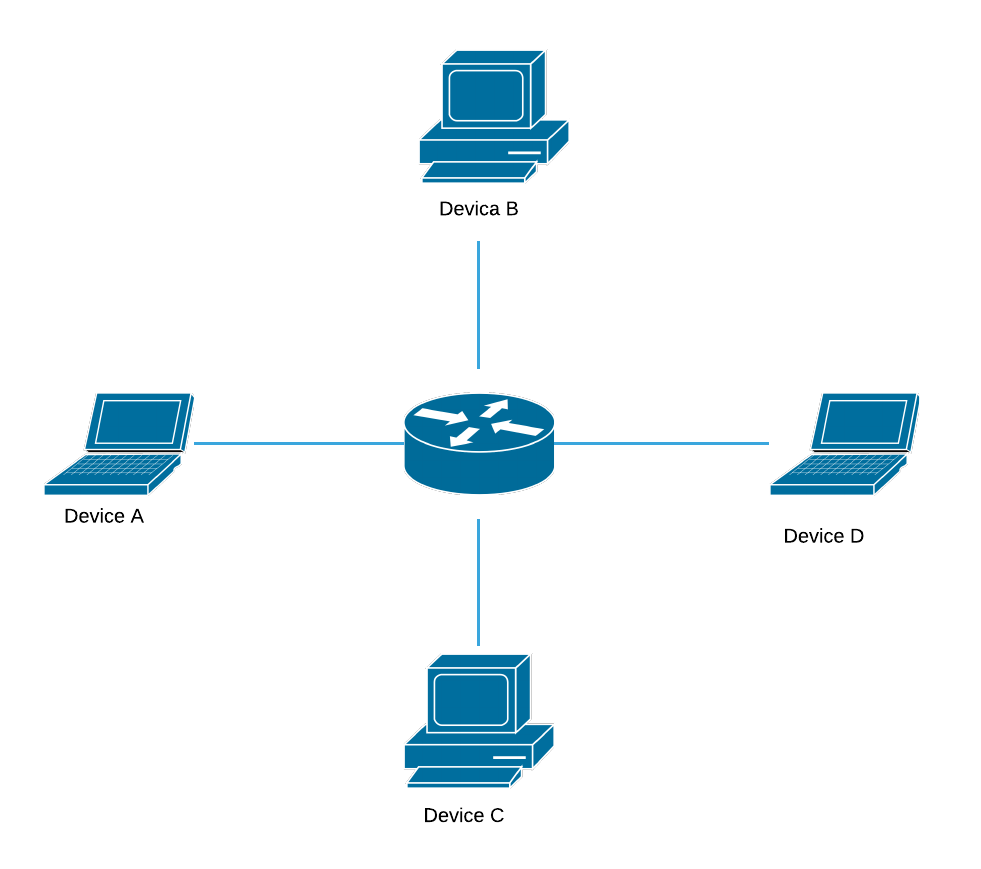
\includegraphics[scale=0.35]{Topology_2} \label{topology_2}}
	\hspace{1cm}
	\subfloat[]{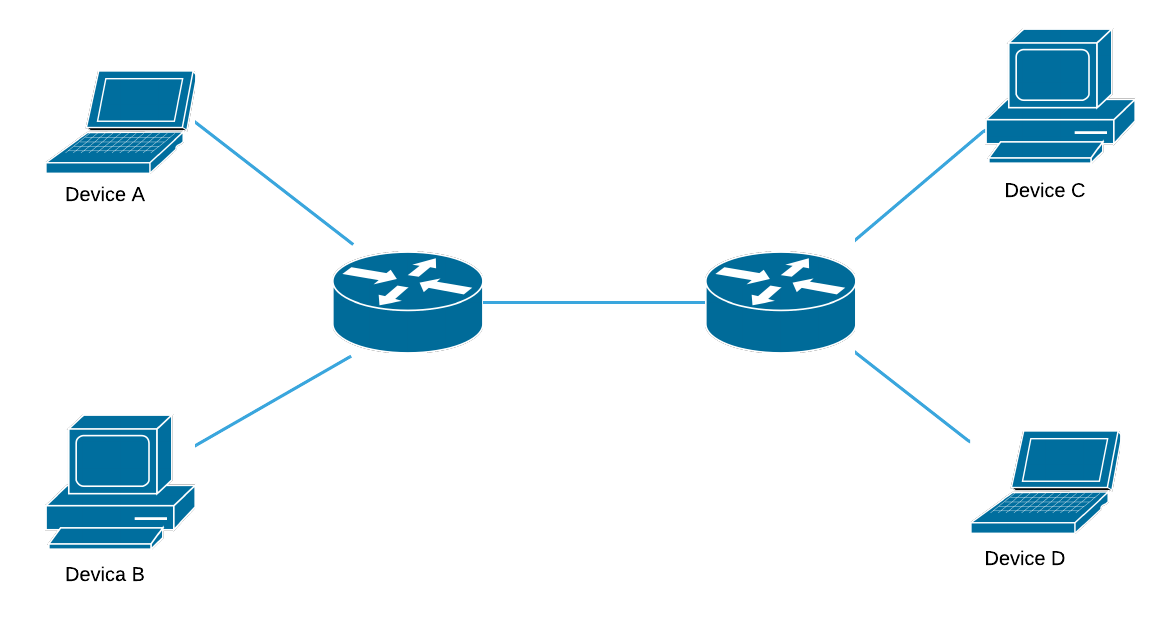
\includegraphics[scale=0.35]{Topology_3} \label{topology_3}}
	\caption{Improvement Topology}
	\label{topology_improvement}
\end{figure}
However, this topology also has the following drawbacks:
\begin{enumerate}
	\item The central device is easy to be overload if there are too many devices connect to it.
	\item It will cost a lot if there are several devices located far away from this central device, \textsl{e.g.} if device C and D is far away from central device, then, the cost to link central device with C and D will be pretty high.
\end{enumerate}
The solution for these two problems is straightforward: By adding more extra devices, as illustrated in Figure \ref{topology_3}. In which, we can assume that device A(C) and B(D) locate in the same area and have relative short distance. Particularly, we can assume device A and B are the computers in one building and device C and D are computers in the other, therefore, we can first connect A, B with one added device and C, D with the other. After that, we can connect these two added devices with each other and hence connect the whole network. Compare with the topology in Figure \ref{topology_2}, this topology has the advantages:
\begin{enumerate}
	\item Is much cheaper as there is only one long-distance connection which happen between the two added devices.
	\item Is much stable as the two added devices do not need to take too much workload compare with the central device in Figure \ref{topology_2}.
\end{enumerate}
Particularly, these added devices, in both Figure \ref{topology_2} and \ref{topology_3}, are called Router and will be explained in further sections. Additionally, the single message that is delivered is called package in terms of Computer Network. 

By the end of this section, we can conclude that the media in Physical Layer is responsible for transferring the message by using its' physical property. However, we still need to define some further mechanisms that control how the message will be delivered, which is the purpose of \textit{Data-Link Layer}. Before we go into these detail, we will first introduce some more high-level thing relate to Computer Network.

Even though the connection between two devices within Network may be complicate, \textsl{e.g.} went through many middle devices like Figure \ref{topology_3}, we can abstract this complicate connection as a direct link that connect the two device and handle the message transportation task, as shown in Figure \ref{virtual}:
\begin{figure}[ht]
	\center
	\subfloat[Real Connection between Two Devices]{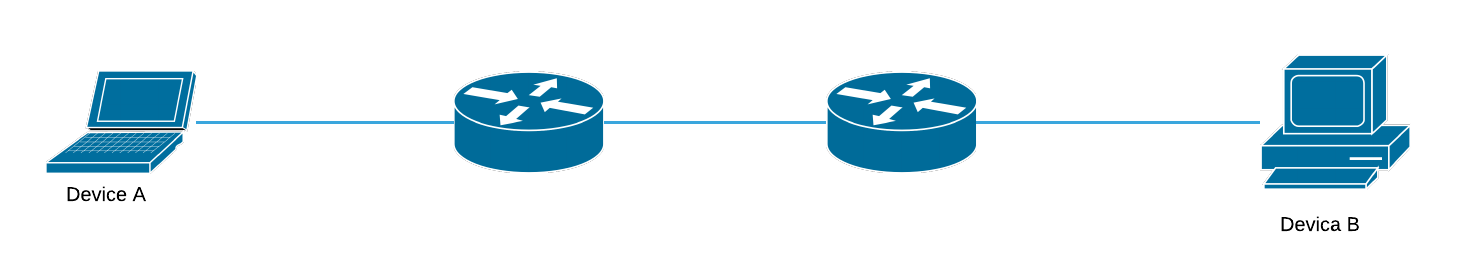
\includegraphics[width = 0.5\textwidth]{Real_Link}  \label{real_link}}
	\vspace{1cm}
	\subfloat[Virtual Connection between Two Devices]{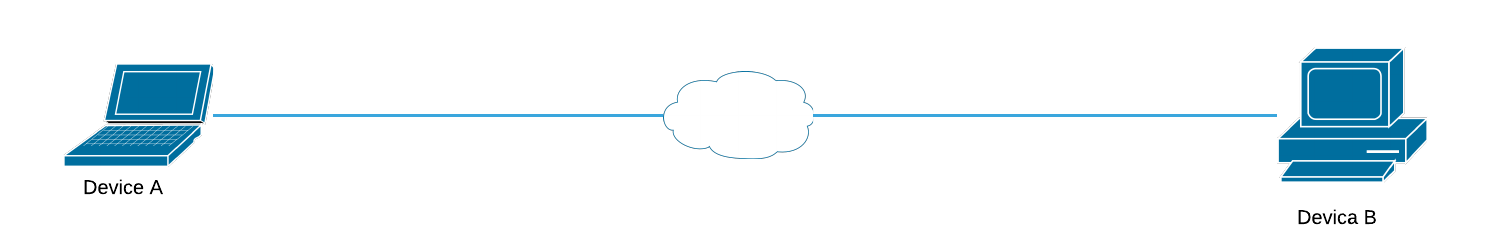
\includegraphics[width=0.55\textwidth] {Virtual_Link} \label{virtual_link}}
	\caption{Virtual Link}
	\label{virtual}
\end{figure}
Figure \ref{real_link} show the real connection between device A and B, which contain two Routers. Figure \ref{virtual_link} abstract this connection as a virtual link. Therefore, from device A and B's perspective, they are directly connecting with each other. Indeed, this virtual link, or we can say, the transportation service provided by the real connection, has the following characteristics to measure it performance:
\begin{enumerate}
	\item \textbf{Reliable}: Measure the frequency of the error that happened during the transmission.
	\item \textbf{Throughput}: Measure the maximum number of packages that can be delivered through this link per second.
	\item \textbf{Delay}: Measure the time that one package transported from one device to the other should take.
\end{enumerate}
This concept of virtual link allow the application within devices do not need to worry about the message transmission, instead, the application can focus on the generation and processing of messages. 
Indeed, one kind of communication that usually happen within Network is that: One device request a file that store in other device. In this case, the device that send the request is called \textit{client} and the device that store the file is called \textit{server}. The communication process is straightforward: The client first send the request to server and the server response with the corresponding file. However, for some servers, it may need to process huge number of request, which will easily cause the server overload. Therefore, an improvement architectural of server is required to handle this problem.

\section{3-Tier Server Architectural}
As mentioned in last part, some server may need to process a lot messages. Therefore, one single device is not enough under this situation as single device do not have ability to handle so much request. One solution is by adding more devices and separate the server into 3 part, in which, each part is corresponding to a specific task, as illustrated in Figure \ref{server}:
\begin{figure}[ht]
	\center
	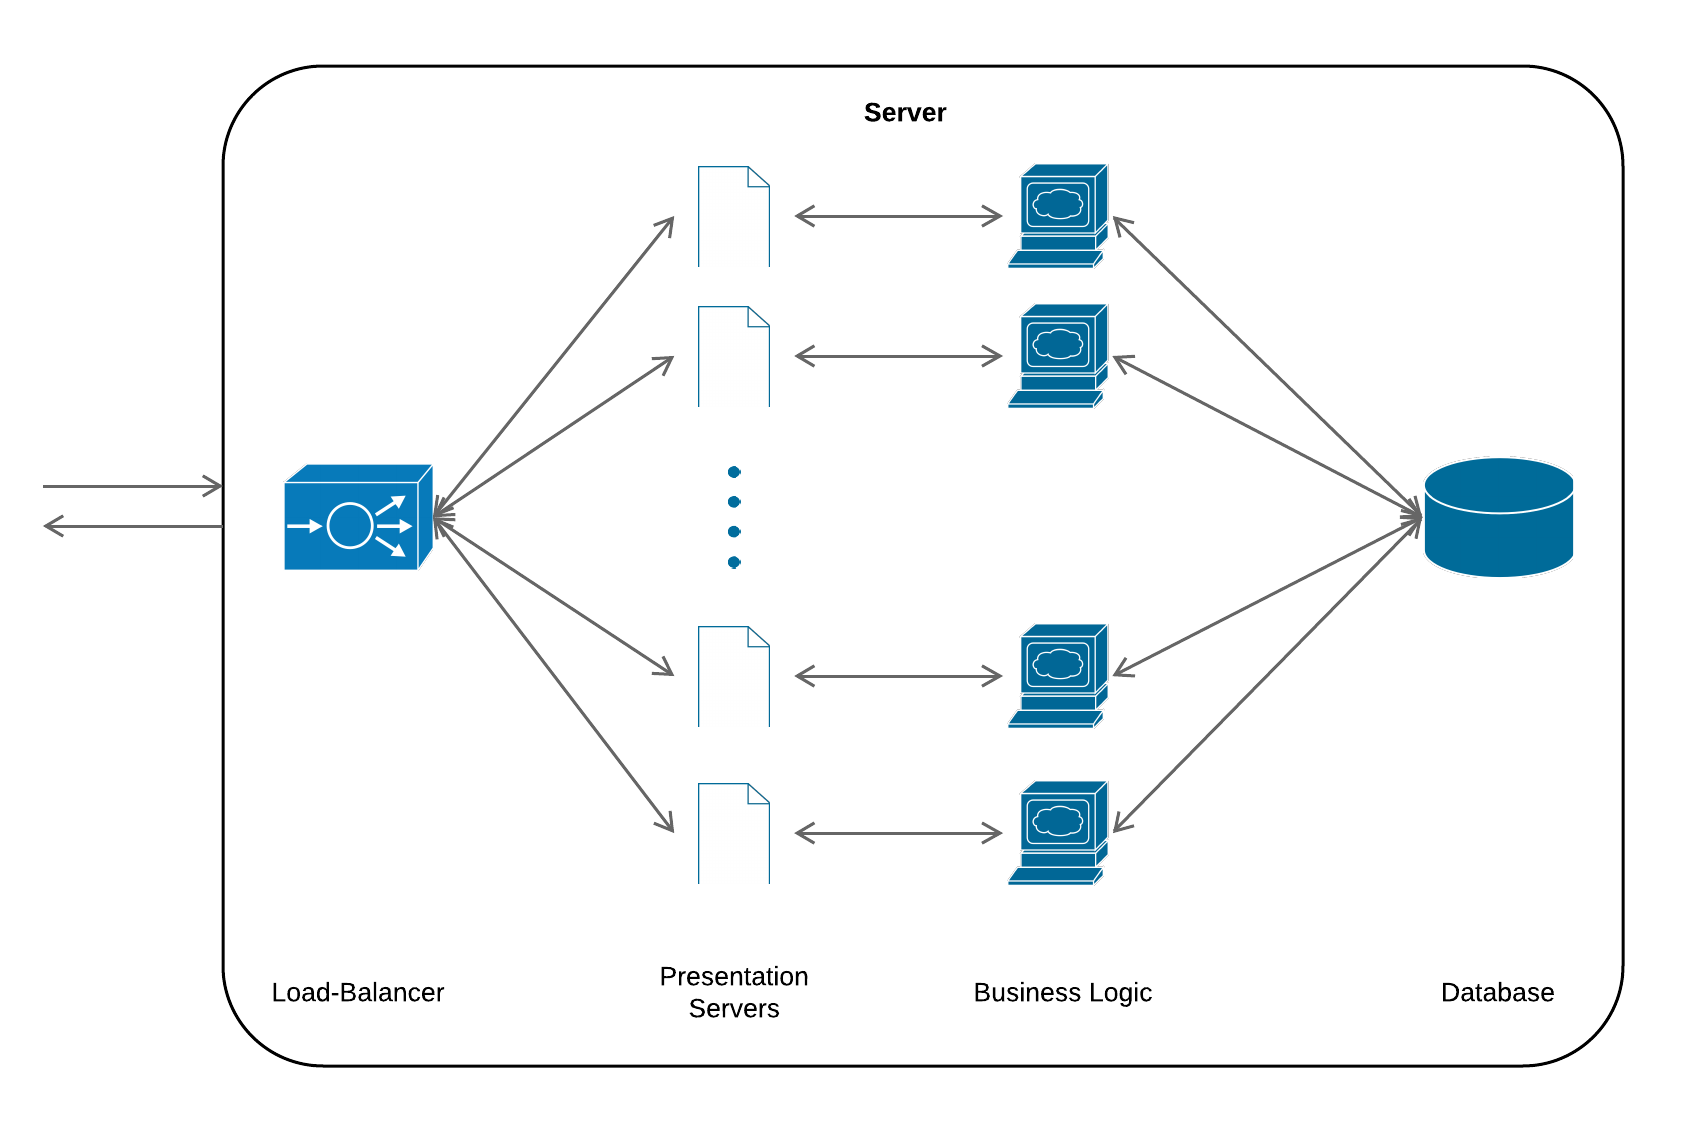
\includegraphics[scale=0.35]{Server}
	\caption{3-Tier Architectural}
	\label{server}
\end{figure}
In which, the server is divided into 3 part in addition to a database:
\begin{enumerate}
	\item \textbf{Load-Balancer}: The load-balancer will assign the coming request to a \textit{Presentation Server} to be further processed.
	\item \textbf{Presentation Server}: The Presentation Server is used to generate the file that requested by coming message.
	\item \textbf{Business Logic Device}: The Business Logic is used to gather and process the data that may used to generate the requested file.
\end{enumerate}
The general process when the server receive a request is:
\begin{enumerate}
	\item The Load-Balancer will first deliver the request to one of the Presentation Servers.
	\item The Presentation Server will ask Business Logic to provide the data that is required for generating file.
	\item The Business Logic will start to gather and process data, \textsl{e.g.} retrieve data from database. 
	\item The Business Logic provide the required data to Presentation Server.
	\item The Presentation Server generate the file by using these data and send it back to Load-Balancer.
	\item  The Load-Balancer send the file back to the client.
\end{enumerate}
Particularly, the database is not count as the part of 3-Tier Server Architectural.
\end{comment}
\end{document}